\documentclass[12pt,a4paper]{article}
\usepackage[utf8]{inputenc} % sempre salve seus arquivos como UTF8
\usepackage[T1]{fontenc}
\usepackage[english]{babel}

\usepackage[left=2.5cm,right=2cm,top=2cm,bottom=2.5cm]{geometry}
\usepackage{amsmath}
\usepackage{amsthm}
\usepackage{amsfonts}

\usepackage{graphicx}
\usepackage{algorithm}
\usepackage{color}
\usepackage[noend]{algpseudocode}
\usepackage{mathtools}
\usepackage{subfig}
\usepackage{diagbox}

% load times font
\usepackage{mathptmx}
\usepackage[scaled=.90]{helvet}
\usepackage{courier}

% comandos
\newcommand{\mdc}[1]{\mathrm{mdc}(#1)}

\DeclarePairedDelimiter\ceil{\lceil}{\rceil}
\DeclarePairedDelimiter\floor{\lfloor}{\rfloor}

% Foot without marker
\newcommand\blfootnote[1]{%
	\begingroup
	\renewcommand\thefootnote{}\footnote{#1}%
	\addtocounter{footnote}{-1}%
	\endgroup
}

\title{MO446 -- Introduction to Computer Vision  \\ Project 3}
\author{Breno Leite  \\ Guilherme Leite}
\date{05/10/2017}

\begin{document}

\maketitle
\blfootnote{\textit{\textbf{Important note:} The borders seen in the figures are not part of the image, they are figurative information about the starting and ending points of the image. Moreover, all the image scales in this report were changed in order to make the text more readable.}} \\

%% ---------------- Starts here --------------------------------

\textbf{\LARGE Question 2 - Data} \\

	The data used in this project was obtained with a cellphone camera recording ordinary objects. Two videos were used, (\textbf{p3-1-0}) shows a translation movement  (affine transformation) of a magic cube in a "blank" background and was used in the experiments of Question 4 - Feature Tracking, (\textbf{p3-1-1}) shows a rotation movement of the same magic cube and was used in Question 5 - Structure from Motion.\\

\textbf{\LARGE Question 3 - Keypoint Selection} \\

	The keypoint selectors explored in this project were Harris and SIFT selector, the most noticeable difference between them is the amount of keypoints extracted, the SIFT algorithm extracts way more keypoints than Harris, and at first glance could be thought as the best choice, more keypoints means a better flow generation, right?

\begin{figure}[!h]
	\centering
	\subfloat[Using Harris. (\textbf{p3-3-1})]{
		{
			\setlength{\fboxsep}{1pt}
			\setlength{\fboxrule}{1pt}
			\fbox{\includegraphics[scale=0.35]{output/p3-3-0}}
		}
		\label{fig:keypointSelectionHarris}
	}
	\quad
	\subfloat[Using SIFT. (\textbf{p3-3-0})]{
		{
			\setlength{\fboxsep}{1pt}
			\setlength{\fboxrule}{1pt}
			\fbox{\includegraphics[scale=0.35]{output/p3-3-1}}
		}
		\label{fig:keypointSelectionSift}
	}
	\caption{Difference between the keypoint selection methods.}
	\label{fig:keypointSelection}
\end{figure}

	Not quite, as the goal is to extract keypoints only from the object and SIFT extracts extra points, seen circled in Figure \ref{fig:keypointSelectionSiftPoints}, like shadows, the line pulling the cube and small light changes, the selector falls behind when compared with the Harris which is a way faster algorithm as shown in Table \ref{table:timeHarrisSift}, and is able to extract only the keypoints regarding the object accomplishing our goal at this stage, as seen in Figure \ref{fig:keypointSelectionHarris}.

\begin{figure}[!h]
	\centering
	{
		\setlength{\fboxsep}{1pt}
		\setlength{\fboxrule}{1pt}
		\fbox{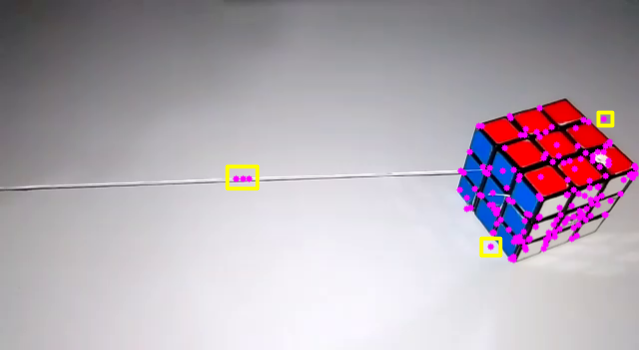
\includegraphics[scale=0.4]{report/out_points}}
	}
	\caption{SIFT extra keypoints.}
	\label{fig:keypointSelectionSiftPoints}
\end{figure}

\begin{table}[!h]
	\centering
	\begin{tabular}{|c|c|c|c|}
		\hline
		& \multicolumn{3}{c|}{\textbf{Time (seconds)}} \\ \hline
		\backslashbox{\textbf{Average of}}{\textbf{Selector}}    & \textbf{Harris}         & \textbf{SIFT}          & \textbf{-1}      \\ \hline
		\textbf{5 runs}  & 0.0067      & 0.0736      & -1     \\ \hline
		\textbf{-1} & -1      & -1       & -1     \\ \hline
	\end{tabular}
	\caption{Comparison between our implementation and OpenCV convolution time.}
	\label{table:timeHarrisSift}
\end{table}

\textbf{\LARGE Question 4 - Feature Tracking} \\

\textbf{\LARGE Question 5 - Structure from Motion} \\

\end{document}
